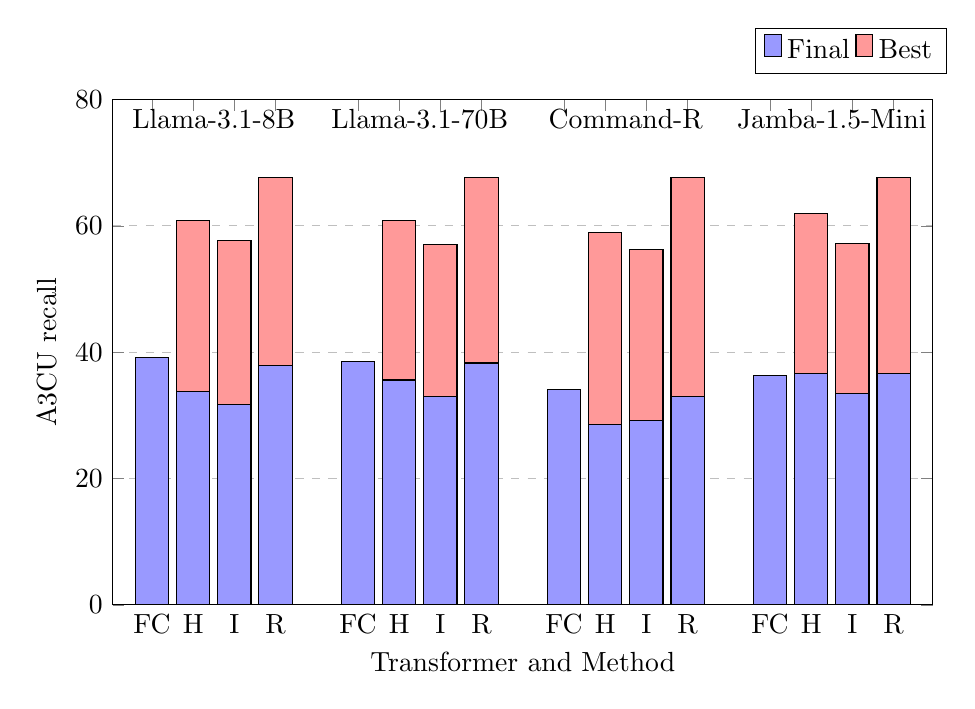
\begin{tikzpicture}
    \begin{axis}[
     width=12cm,
     height=8cm,
     ybar stacked,
     bar width=12pt,
     ylabel={A3CU recall},
     xlabel={Transformer and Method},
     xticklabels={
     FC, H, I, R,
     FC, H, I, R,
     FC, H, I, R,
     FC, H, I, R
     },
     xtick={0,1,2,3,5,6,7,8,10,11,12,13,15,16,17,18},
     x tick label style={anchor=north},
     legend style={at={(0.9,1.05)},anchor=south,legend columns=-1},
     ymajorgrids=true,
     grid style=dashed,
     ymin=0,
     ymax=80,
     enlarge x limits={abs=0.5cm},
    ]
    \addplot[fill=blue!40] coordinates {
     (0,39.1) (1,33.8) (2,31.7) (3,37.9)
     (5,38.6) (6,35.6) (7,33.0) (8,38.3)
     (10,34.1) (11,28.6) (12,29.2) (13,33.0)
     (15,36.3) (16,36.6) (17,33.4) (18,36.6)
     };
    \addplot[fill=red!40] coordinates {
     (0,0) (1,27.0) (2,26.0) (3,29.7)
     (5,0) (6,25.2) (7,24.1) (8,29.3)
     (10,0) (11,30.4) (12,27.0) (13,34.6)
     (15,0) (16,25.4) (17,23.8) (18,31.0)
     };
    \legend{Final, Best}
    \node[anchor=north] at (axis cs:1.5,80) {Llama-3.1-8B};
    \node[anchor=north] at (axis cs:6.5,80) {Llama-3.1-70B};
    \node[anchor=north] at (axis cs:11.5,80) {Command-R};
    \node[anchor=north] at (axis cs:16.5,80) {Jamba-1.5-Mini};
    \end{axis}
\end{tikzpicture}